\chapter{Evaluation}

\section{User Experience}
Der erste Punkt, der evaluiert werden muss, ist, ob die Anwendung in ihrer jetzigen Form von der Zielgruppe verstanden wird. Dabei muss zum einen die Bedienung der Anwendung als Ganzes überprüft werden. Dazu zählt zum einen, dass das User Interface ohne Erklärungen bedient werden kann und bestimmte Aufgaben aus dem Use Case erfüllt werden können. Zum anderen muss die Visualisierung korrekt interpretiert werden können. Hier ist zum Beispiel zu prüfen, ob der Benutzer von Anfang an die Farben einzelnen Höhenwerten zuordnen kann. Auch die Kamerasteuerung ist ein wichtiger Aspekt, der hier überprüft werden muss. Hier sollte geprüft werden, welche der beiden Kameraimplementationen vom User bevorzugt wurden und ob beide Implementationen zur Erfüllung des Use Case nützlich waren. Auch bestimmte Details wie das Dragging der Maus zum Umsehen wurde während des Projekts als potentiell erklärungsbedürftig eingestuft, muss hier also überprüft werden. Neben der Intuitivität muss auch überprüft werden, wie gut der User mit der Kamera zurecht kommt. Hier ist wichtig, dass der Nutzer sowohl bei hohen Zoomstufen als auch aus großer Entfernung flüssig bestimmte Orte an navigieren kann. Hier ist die Sorge, dass die Geschwindigkeit der Kamera bei einer geringen Distanz zu groß ist, insbesondere bei der rotierenden Kamera. Mit der frei bewegbaren Kamera ist die Idee, dass sich bestimmte Punkte leichter erreichen lassen, da hier die laterale Bewegungen (Steuerung der Blickrichtung) linear abhängig von der Mausbewegung ist, welche in der Regel sehr präzise sein kann. Schlussendlich muss überprüft werden, welche Auswirkungen die Techniken zur Datenreduktion auf die User Experience haben. Dazu soll geprüft werden, in weit die Tester das Nachladen von Abschnitten wahrnehmen, bzw. wie störend sie es empfinden. Idealerweise sollten natürlich keine Ladeartefakte zu sehen sein, dies kann auf Grund eigener Tests jedoch ausgeschlossen werden. Außerdem ist zu ermitteln, ob die Tester die dynamischen Auflösungsanpassungen wahrnehmen können.

Die Durchführung der Evaluation gestaltete sich auf Grund der aktuellen Covid-19 Pandemie als sehr schwierig. Insgesamt konnten nur vier Personen aus der Zielgruppe gefunden werden, die die Anwendung testeten. Dies reicht natürlich nicht aus, um eine repräsentative Meinung dazu zu erhalten, allerdings reichte es, um einige Probleme mit der Anwendung aufzudecken. Als erstes wurde die Anwendung unter einer öffentlichen Domain gehosted, sodass der Zugang kein Spezialwissen über den Build-Prozess benötigte. Anschließend wurde ein Fragebogen übermittelt, der die oben genannten Punkte abdeckte. Hier wurde als erstes ein Use Case definiert, den die Benutzer abzuarbeiten hatten. Konkret sollte mit Hilfe aller Features der höchste Punkt auf dem Mars gefunden werden. Die Idee dahinter war, dass der Nutzer an Hand der Farben relativ schnell einen hohen Punkt findet, den Höhenwert an Hand des Klicks auf den Globus ermittelt und im Konfigurationsmenü daraufhin die Skala so anpasst, dass kleinere Werte nicht mehr beachtet werden. Dieser Prozess, welcher leicht an eine Binärsuche erinnert, sollte dann iterativ wiederholt werden. Die Benutzer bekamen dabei natürlich keine Erklärungen und die Erwartung war auf Grund eigener Tests um die zwei oder drei Iterationen. Dieser Use Case involviert die Zusammenarbeit verschiedener Features und testet, ob der Nutzer die Visualisierung einordnen kann. Insbesondere wurde damit auch der kritische Punkt abgedeckt, dass die Erklärung des Höhenmessfeatures nirgendwo beschrieben und seine Indikation während des Projekts als zweifelhaft eingestuft wurde. Die Benutzer nahmen dann eine Bewertung auf dem Fragebogen vor, wobei hier oftmals eine Skala genutzt wurde um festzustellen, wie gut der Tester dies erfüllen konnte oder wie gut er mit der jeweiligen Interaktion zurecht kam.

Den gestellten Use Case konnten alle Tester relativ gut erfüllen. Hier ist festzuhalten, dass die Genauigkeit relativ stark schwankte und einige Tester sich dabei mehr oder weniger Mühe gegeben hatten, den Punkt auch wirklich genau zu finden. Alle fanden jedoch die ungefähre Umgebung und einen recht hohen Höhenwert. Auch ist wichtig, dass alle Tester zumindest einmal die Skala anpassten, da sie feststellten, dass die Skala in ihrer Standardkonfiguration nicht ausreichte um den höchsten Punkt zu finden. Alle Tester fanden ohne Erklärung heraus, wie die Position und die Höhe eines Punktes ermittelt werden kann und wo dies angezeigt wird. Hier war die Sorge also unbegründet und es muss keine weitere Verbesserung vorgenommen werden. Für die Erfüllung des Use Case nutzen alle Tester die gleiche rotierende Standardkamera. Alle konnten diese intuitiv steuern und es gab keine Erklärungsnotwendigkeit beim Dragging. Sie bewerteten die Steuerung hier alle mit der höchsten Punktzahl. Die sich frei bewegende Kamera dagegen wurde weniger gut bewertet und drei der Tester konnten damit sehr schlecht umgehen. Hier wurde vor allem kritisiert, dass es sehr lange dauert, zur anderen Seite des Globus zu gelangen und dass ein Ändern der des Betrachterwinkels auf der y-Achse (Inklanation) sehr schwierig ist. Hier müsste der Nutzer sein Blickwinkel strikt nach oben richten, sich dann leicht vorwärts bewegen und dann wieder den original Blickwinkel einnehmen, ohne das dabei die Position auf der x- oder z-Achse verändert wurde. Hier hätte eine weitere Taste integriert werden können, mit dem man die Kamera entlang der Blickrichtung hoch oder runter bewegen könnte. Im Gegensatz zu den Steuerungstasten WASD oder den Pfeiltasten sind jedoch dafür keine Tasten bekannt, sodass dieses Feature wahrscheinlich nicht ohne Erklärung wahrgenommen wäre. Alle Tester waren schlussendlich der Meinung, dass die frei bewegliche Kamera, zumindest in der Kugelprojektion, nicht hilfreich ist. Die Ansicht ohne Projektion wurde von allen Testern als neutral beurteilt und viele sahen dafür keinen echten Grund. Die Ansicht als Globus wurde jedoch von allen Testern bevorzugt. Die Unterteilung in Abschnitte wurde wie erwartet von allen Testern wahrgenommen und als störend empfunden, sodass hier deutliche Verbesserungen vorgenommen werden müssen. Die Anpassung der Auflösung zur Laufzeit wurde allerdings nicht wahrgenommen, das Tauschen von existierenden Abschnitten zur Laufzeit war also ein Erfolg.

Des Weiteren konnten die Tester allgemeine Kommentare und Verbesserungsvorschläge über die Anwendung abgeben. Hier wurde zum einen mehrmals angemerkt, dass die 3D Darstellung der Oberfläche schlecht zur Geltung kommt. Dies ist natürlich zutreffend, da das Verhältnis von Höhen zum Durchmesser des Planeten natürlich absolut gering ist. Auch die Farben haben hier nicht ausgereicht, um, besonders bei hohen Zoomstufen, einen Höhenunterschied zu simulieren. Für zukünftige Projekte wurde hier geplant einen Konfigurationsparameter hinzuzufügen, der Höhenwerte zusätzlich verstärken kann. So ein Parameter war rückblickend betrachtet auch in einer der analysierten Alternativen zu finden, sodass dies ein Problem darstellt, was bereits bekannt war. Hier muss dann natürlich immer überlegt werden, inwieweit man die Darstellung von einer realistischen Darstellung entfernen will, ein Punkt, der sehr stark vom späteren Use Case abhängt. Außerdem bemängelten die Hälfte der Tester, dass die Farbskala nicht dauerhaft zu sehen war und dass ein dauerhaftes Ausklappen des Informationspanels störend wäre. Hier hätte also eine Trennung stattfinden können, wobei die andere Hälfte dies natürlich als nicht störend empfunden hatte.

\section{Profiling}
Nachdem die Anwendung funktional auf einem akzeptablen Stand war, musste verifiziert werden, dass dies auch für die Performance zutraf. Insbesondere, da diese, auf Grund der Datenmenge, natürlich besonders im Vordergrund steht. Da die Performance natürlich von Testern nicht in ausreichendem Maße ermittelt werden kann, konnte die Performance nur in Eigenanalyse auf einem Satz Hardware durchgeführt werden. Dies ist natürlich nicht ausreichend um die Performance für verschiedene Performanceklassen zu bestimmen. Dies führt auch dazu, dass die Anpassung der Visualisierung an verschiedenste Hardwarebedingungen, wie in den nicht-funktionalen Anforderungen (siehe \ref{nichtFunktional}) beschrieben, nicht getestet werden kann. Konkret dafür genutzt wurde ein Rechner mit einer GeForce GTX 970 Grafikkarte mit 4 GB VRAM, einer Intel i7-4790K 4 GHz CPU und 16 GB DDR3 RAM. Die Anwendung wurde bei allen Tests in Google Chrome 94 getestet. Die maximale Downloadgeschwindigkeit beträgt 100 Mbit/s auf einer DSL Leitung. Alle hier ermittelten Messwerte sind der Durchschnitt aus mehreren Messungen, wobei der Browsercache natürlich nach jedem Durchlauf geleert wurde. Ein Problem beim Profilen der GPU ist, dass es nahezu unmöglich ist, von außen nur die Performancedaten der eigenen Anwendung zu ermitteln. Auf CPU Seite existieren dagegen Threads, welche man unabhängig von den anderen Threads betrachten kann. Viele GPU Profiling Tools nutzen daher das Konzept der Instrumentierung, bei dem der Code mit Analyse Code erweitert wird. Das konnte auf Grund von Zeitgründen bei diesem Projekt nicht durchgeführt werden und im folgenden sind die Daten der GPU durch andere Anwendungen leicht verfälscht.

Die Punkte, welche hier überprüft werden müssen, sind teilweise in den nicht-funktionalen Anforderungen definiert und sind vor allem die Auslastung von Grafik- und Arbeitsspeicher. Diese darf selbst bei vielfachen Benutzeraktionen die Grenze von 4 GB bzw. 8 GB nicht überschreiben. Außerdem ist die erreichte Anzahl an Frames pro Sekunde (FPS) zu ermitteln, womit überprüft werden kann, wie gut der Spagat aus Performance und User Experience gelungen ist. Auch die Auslastung von CPU und GPU zu allen Zeiten ist zwar nicht definiert, sollte jedoch auf einem akzeptablen Maß liegen. Ein weiterer Punkt ist auch die Ladezeit bis zum vollständigen Laden aller Abschnitte in der initialen Ansicht. Dies ist der erste Eindruck eines jeden Nutzers und sollte dementsprechend relativ gut sein. 

Ein erstes Profiling mit Hilfe der Entwicklertools stellte schnell fest, dass die Anwendung weder auf CPU- noch auf GPU-Seite ausgelastet ist. Auf CPU Seite wurde während des gesamten Tests  nur 16\% der Zeit im JavaScript verbracht (siehe Abbildung \ref{cpuUsage}). Auch die Zeit in der GPU stellte mit 3.5\% einen sehr geringen Anteil dar (siehe Abbildung \ref{gpuUsage}). Dies sagt natürlich noch nichts darüber aus, wie stark der Prozessor während einzelner, spezieller Zeiten genutzt wurde. Aber auch dort kann in Abbildung \ref{overallPerformance} gesehen werden, dass nach einer vollen Auslastung beim Laden der Seite jemals wieder eine volle Auslastung erreicht wurde. Auch erreichte sie nach dem initialen laden fast dauerhaft 60 FPS (grüne Linie), was auf dieser Hardware laut den Anforderungen eigentlich zu hoch ist. Es waren zwar einzelne Einbrüche auf 30 FPS zu sehen\footnote{vSync führt hier dank des Wartens auf das nächste Refresh-Intervall zu so einem starken Abfall}, diese können jedoch nicht durch eine besonders starke GPU Auslastung zu bestimmten Frames erklärt werden.

\begin{figure}[H]
  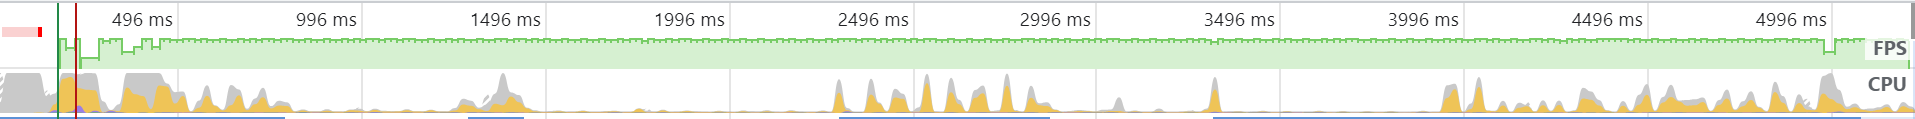
\includegraphics[width=\textwidth]{overallPerformance.png}
  \caption{CPU Auslastung und Framerate über Zeit}
  \label{overallPerformance}
\end{figure}

\begin{figure}[H]
  \begin{minipage}{0.5\textwidth}
    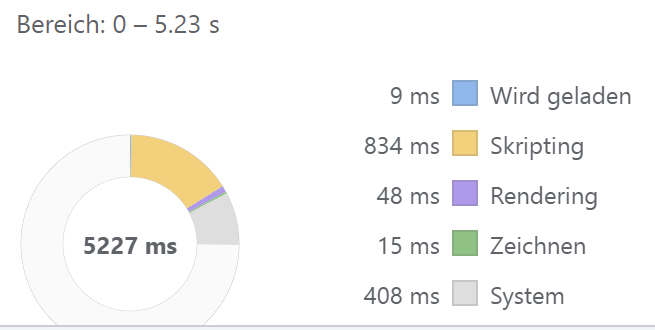
\includegraphics[width=0.95\textwidth]{cpuUsage.png}
    \caption{Totale CPU Auslastung}
    \label{cpuUsage}
  \end{minipage}
  \begin{minipage}{0.5\textwidth}
    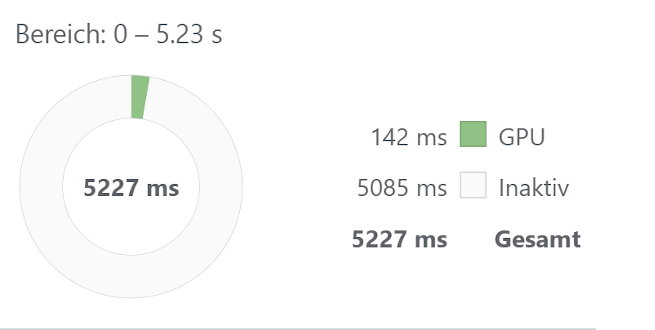
\includegraphics[width=0.95\textwidth]{gpuUsage.png}
    \caption{Totale GPU Auslastung}
    \label{gpuUsage}
  \end{minipage}
\end{figure}

Trotzdem waren bei der Benutzung der Anwendung relativ starke Lade-Artefakte zu sehen. Man konnte das Laden der einzelnen Abschnitte verfolgen und es kam zu spürbaren Verzögerungen zwischen vollständigen Ansichten. Hierzu muss natürlich gesagt werden, dass per starker Kamerabewegungen der Ladeprozess unnatürlich stark beeinflusst wurde. Es wurde sowohl das Laden von neuen Abschnitten als auch die Änderung des Details Grades stark forciert, was nicht einer normalen Nutzung entspricht. Hier wurde festgestellt, dass die Anwendung bei einer so großen Datenmenge durch das Netzwerk ausgelastet ist (siehe Abbildung \ref{requests}).

\begin{figure}[H]
  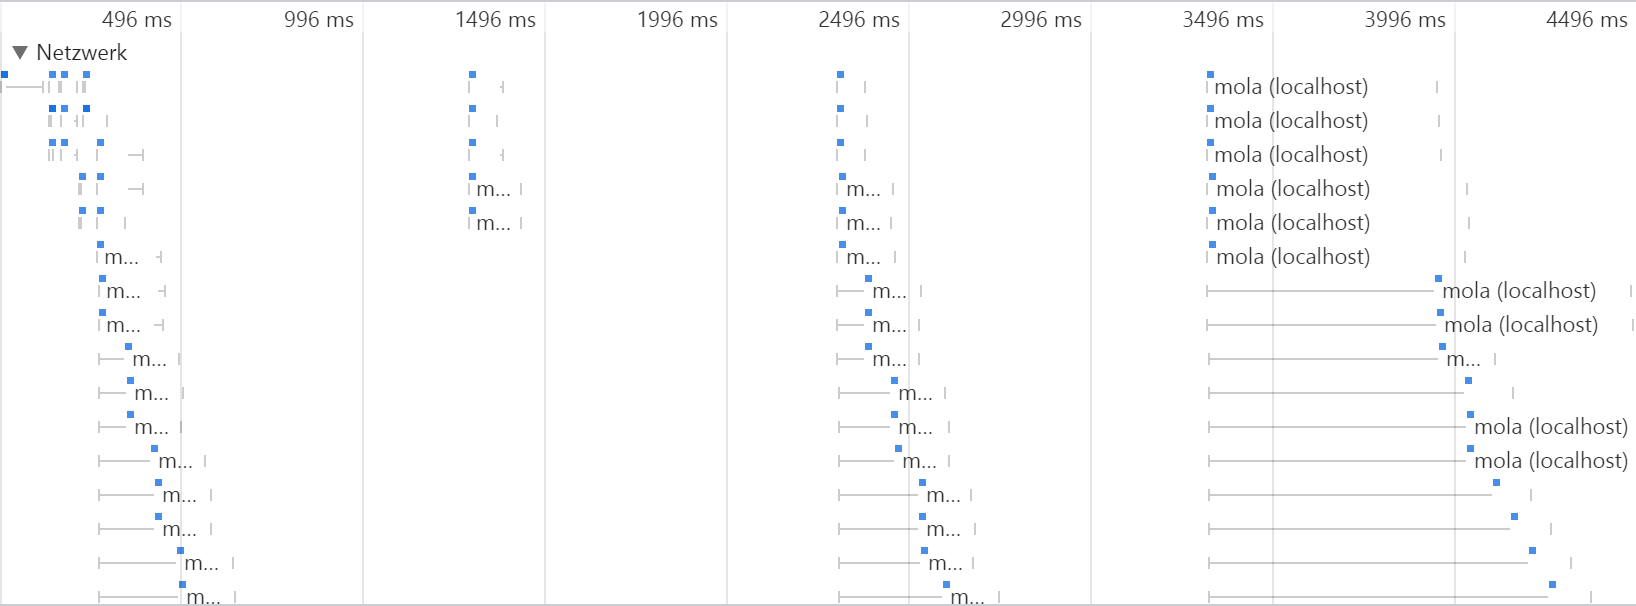
\includegraphics[width=\textwidth]{requests.png}
  \caption{Dauer der Laderequests über Zeit}
  \label{requests}
\end{figure}

Hier sind die Dauer der einzelnen Requests über die Zeit zu sehen und man kann deutlich sehen, dass diese mit der Zeit immer länger dauern. Auch lässt sich deutlich die Drosselung des Ladevorgangs auf jede Sekunde erkennen, da sich alle Requests einer Gruppe mit gleicher Anfangszeit zuordnen lassen. Am Anfang waren diese Requests mit 70 ms bis maximal 150 ms schon relativ hoch. Auch die Dauer einzelner Requests pro Vorgang wuchs an, was darauf hindeutet, dass pro Ladevorgang schneller Requests gesendet wurden, als das diese bearbeitet wurden. Noch kann man allerdings erkennen, dass eine Gruppe vollständig fertig mit Laden ist, bevor der nächste Ladezyklus beginnt. Nach einigen Sekunden steigt die Dauer der Requests dann allerdings plötzlich auf 700 ms bis maximal 1.5 s an, was nicht mehr vertretbar ist. Ab diesem Zeitpunkt überlagern sich dann auch die Ladezyklen (siehe Abbildung \ref{requestOverlap}). 

\begin{figure}[H]
  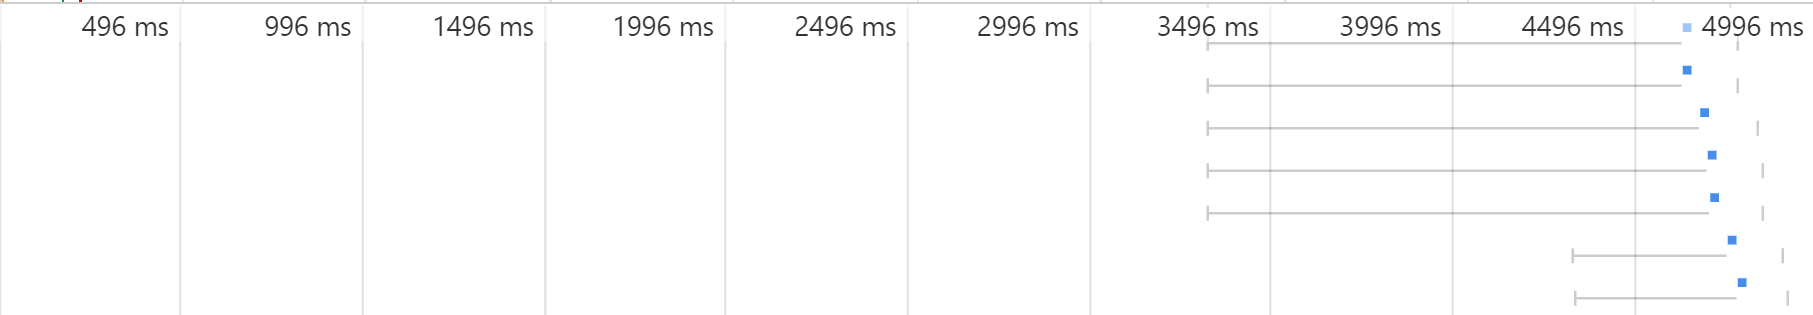
\includegraphics[width=\textwidth]{requestOverlap.png}
  \caption{Überlappen von Ladezyklen}
  \label{requestOverlap}
\end{figure}

Dies ist ein nicht hinnehmbarer Zustand, da ab diesem Zeitpunkt ein kritischer Punkt erreicht ist, ab dem sich alle Requests mit fortlaufender Zeit immer mehr anstauen. Jetzt ist natürlich die Frage, ob diese Limitierung auf Grund der begrenzten Bandbreite und hoher Datenmenge auftritt oder ob der Webserver seine maximale Kapazität erreicht hat. Auf Seiten des Webservers könnte zum einen die Menge an Requests ein limitierender Faktor sein. Zum anderen könnte die Engstelle beim Zugriff auf die Datei mit den Quelldaten liegen, da diese ja für jede Anfrage neu ausgelesen werden muss. Ein Profiling des Server ergab allerdings keine Performanceprobleme. Es standen ungenutzte Threads zur Verfügung und auch die CPU Auslastung war nicht besorgniserregend. Der Durchsatz des Dateisystems lässt sich relativ schwer bestimmen, allerdings wurde es als unwahrscheinlich eingestuft. Klarheit ergab dann der genauere Blick auf einen der am längsten laufende Requests (siehe Abbildung \ref{specificRequest}).

\begin{figure}[H]
  \centering
  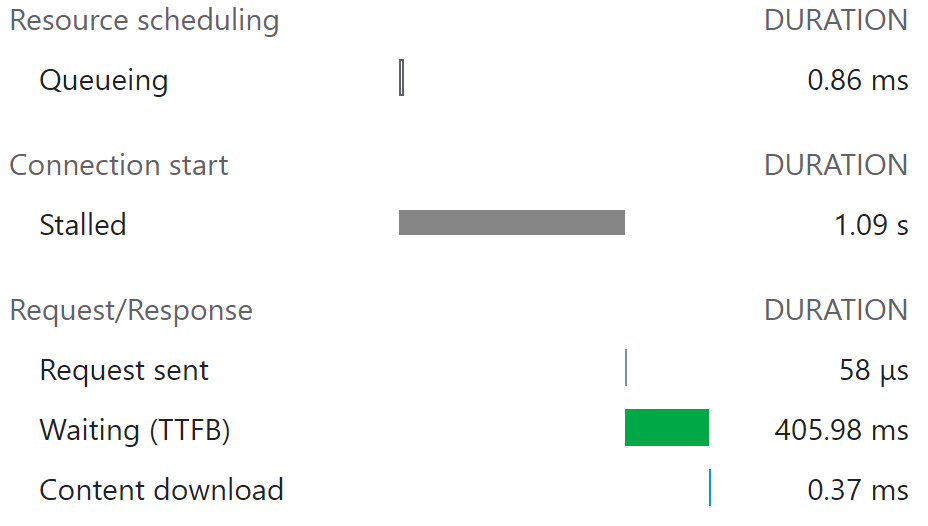
\includegraphics[width=0.7\textwidth]{specificRequest.png}
  \caption{Details des am längsten laufenden Requests}
  \label{specificRequest}
\end{figure}

Dies zeigt, dass der Requests auf Client-Seite sehr lang im Status “Stalled” wartete. Die Zeit, welche mit dem Warten auf die Antwort verbracht wurde, machte dabei nur ein Drittel der Gesamtzeit aus. Eine kurze Recherche zeigte dann, dass die maximale Anzahl an nebenläufigen Requests pro Server im Google Chrome Browser auf sechs limitiert ist. Auch wenn also auf dem Server genügend Ressourcen verfügbar sind, werden diese nicht vollständig ausgeschöpft. Dieses Limit des Browsers lässt sich trotz vielfältiger Feature Requests\footnote{z.B. https://bugs.chromium.org/p/chromium/issues/detail?id=87381} nicht ändern. Als einziger Optimierungspunkt bleibt also die Reduzierung der Laufzeit einzelner Requests auf Serverseite, was nicht trivial umsetzbar ist. Auch könnte man überlegen das HTTP/2 Server Push Feature zu nutzen, mit dem ein Server auf einen Request mit mehr als nur einer Response antworten kann. Somit könnte die Limitierung der Anzahl der Requests umgangen werden. Es ist jedoch unklar, wie aufwändig eine dementsprechende Änderung auf Client- und Serverseite ist.

Auch der Speicherverbrauch im RAM ist deutlich unter den Erwartungen und den Anforderungen. Der Graph zeigt den Speicherplatz im JavaScript Heap über die Zeit an. Die Werte schwanken dabei zwischen 1.1 MB und 9.5 MB.

\begin{figure}[H]
  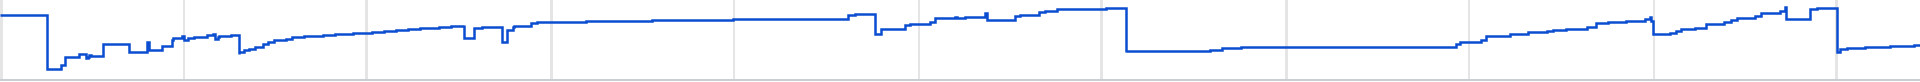
\includegraphics[width=\textwidth]{heapSize.png}
  \caption{Speicherverbrauch im JavaScript Heap über Zeit}
  \label{specificRequest}
\end{figure}

Der gesamte RAM und VRAM wurde auch in den Abbildung \ref{memoryAvg} und \ref{memoryMax} mit dem Tool gpu-z ermittelt. Da dies natürlich systemweite Werte darstellt, kann nur mit der Differenz zum Startzeitpunkt gearbeitet werden, um damit einen ungefähren Wert zu erhalten. Dieser Wert ist natürlich auch durch die Benutzung des Browsers an sich verfälscht. Zu Beginn des Tests war der VRAM mit 840 MB und der RAM mit 7740 MB gefüllt. Der Memory Controller Load kann als Indiz genutzt werden, mit welchem Durchsatz Daten auf die GPU geschafft werden können. Seine Auslastung lag zu Anfang bei 2\%. Die GPU Auslastung wurde hier auch nochmal betrachtet, da vorige Tests nur die totale Zeit auf der GPU betrachtet hatten, was nichts darüber aussagt, wie stark sie zu bestimmten Zeiten beansprucht wurde. Da eine GPU eine geteilte Ressource ist, sollte man hierbei auch an andere Anwendungen denken. Sie lag zu Beginn des Tests bei ungefähr 5\%.

\begin{figure}[H]
  \begin{minipage}{0.5\textwidth}
    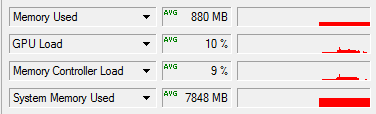
\includegraphics[width=0.95\textwidth]{memoryAvg.png}
    \caption{Durchschnittlicher Speicherverbrauch und Auslastung}
    \label{memoryAvg}
  \end{minipage}
  \begin{minipage}{0.5\textwidth}
    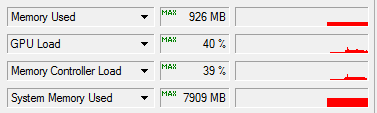
\includegraphics[width=0.95\textwidth]{memoryMax.png}
    \caption{Maximaler Speicherverbrauch und Auslastung}
    \label{memoryMax}
  \end{minipage}
\end{figure}

Auch dieser Test zeigt eine durchschnittliche RAM Nutzung von 108 MB und eine maximale Nutzung von 169 MB, was sich zwar von vorigen Messungen unterschiedet, aber immer noch stark unter den Anforderungen ist. Auch die durchschnittliche VRAM Nutzung von 40 MB und die maximale Nutzung von 86 MB ist nicht zu beanstanden. Interessant ist noch die maximale GPU Auslastung von 40\%, welche deutlich über dem Durchschnitt von 10\% liegt. Dies zeigt aber auch nur, dass selbst zu kritischsten Zeiten die Auslastung völlig vertretbar ist. Und schlussendlich zeigt der maximale Memory Controller Load von 39\%, dass der Datendurchsatz in zukünftigen Projekten mehr als verdoppelt werden könnte.

Als letzten Punkt wurden die Ladezeiten betrachtet, welche auf Grund des asynchronen Natur des Laden schwer zu ermitteln waren. Hier wurde der Ladevorgang um Timing Informationen erweitert um so einen ungefähren Überblick zu erhalten. Nach dem Neuladen der Seite dauerte es dabei 746 ms ab dem onload-Event des Browsers, bis alle Abschnitte in der initialen Ansicht geladen waren. Das onload-Event wird vom Browser gesendet, nachdem alle statischen Ressourcen (HTML, Scripte, Bilder, etc.) geladen wurden. Es trat laut den Entwicklertool nach 112 ms auf, was zu einer gesamten Ladezeit von 858 ms führt. Eine Ladezeit von unter einer Sekunde wurde auf Grund der Datenmenge als vertretbar eingestuft.